% GNUPLOT: LaTeX picture with Postscript
\begingroup
  \makeatletter
  \providecommand\color[2][]{%
    \GenericError{(gnuplot) \space\space\space\@spaces}{%
      Package color not loaded in conjunction with
      terminal option `colourtext'%
    }{See the gnuplot documentation for explanation.%
    }{Either use 'blacktext' in gnuplot or load the package
      color.sty in LaTeX.}%
    \renewcommand\color[2][]{}%
  }%
  \providecommand\includegraphics[2][]{%
    \GenericError{(gnuplot) \space\space\space\@spaces}{%
      Package graphicx or graphics not loaded%
    }{See the gnuplot documentation for explanation.%
    }{The gnuplot epslatex terminal needs graphicx.sty or graphics.sty.}%
    \renewcommand\includegraphics[2][]{}%
  }%
  \providecommand\rotatebox[2]{#2}%
  \@ifundefined{ifGPcolor}{%
    \newif\ifGPcolor
    \GPcolortrue
  }{}%
  \@ifundefined{ifGPblacktext}{%
    \newif\ifGPblacktext
    \GPblacktexttrue
  }{}%
  % define a \g@addto@macro without @ in the name:
  \let\gplgaddtomacro\g@addto@macro
  % define empty templates for all commands taking text:
  \gdef\gplbacktext{}%
  \gdef\gplfronttext{}%
  \makeatother
  \ifGPblacktext
    % no textcolor at all
    \def\colorrgb#1{}%
    \def\colorgray#1{}%
  \else
    % gray or color?
    \ifGPcolor
      \def\colorrgb#1{\color[rgb]{#1}}%
      \def\colorgray#1{\color[gray]{#1}}%
      \expandafter\def\csname LTw\endcsname{\color{white}}%
      \expandafter\def\csname LTb\endcsname{\color{black}}%
      \expandafter\def\csname LTa\endcsname{\color{black}}%
      \expandafter\def\csname LT0\endcsname{\color[rgb]{1,0,0}}%
      \expandafter\def\csname LT1\endcsname{\color[rgb]{0,1,0}}%
      \expandafter\def\csname LT2\endcsname{\color[rgb]{0,0,1}}%
      \expandafter\def\csname LT3\endcsname{\color[rgb]{1,0,1}}%
      \expandafter\def\csname LT4\endcsname{\color[rgb]{0,1,1}}%
      \expandafter\def\csname LT5\endcsname{\color[rgb]{1,1,0}}%
      \expandafter\def\csname LT6\endcsname{\color[rgb]{0,0,0}}%
      \expandafter\def\csname LT7\endcsname{\color[rgb]{1,0.3,0}}%
      \expandafter\def\csname LT8\endcsname{\color[rgb]{0.5,0.5,0.5}}%
    \else
      % gray
      \def\colorrgb#1{\color{black}}%
      \def\colorgray#1{\color[gray]{#1}}%
      \expandafter\def\csname LTw\endcsname{\color{white}}%
      \expandafter\def\csname LTb\endcsname{\color{black}}%
      \expandafter\def\csname LTa\endcsname{\color{black}}%
      \expandafter\def\csname LT0\endcsname{\color{black}}%
      \expandafter\def\csname LT1\endcsname{\color{black}}%
      \expandafter\def\csname LT2\endcsname{\color{black}}%
      \expandafter\def\csname LT3\endcsname{\color{black}}%
      \expandafter\def\csname LT4\endcsname{\color{black}}%
      \expandafter\def\csname LT5\endcsname{\color{black}}%
      \expandafter\def\csname LT6\endcsname{\color{black}}%
      \expandafter\def\csname LT7\endcsname{\color{black}}%
      \expandafter\def\csname LT8\endcsname{\color{black}}%
    \fi
  \fi
    \setlength{\unitlength}{0.0500bp}%
    \ifx\gptboxheight\undefined%
      \newlength{\gptboxheight}%
      \newlength{\gptboxwidth}%
      \newsavebox{\gptboxtext}%
    \fi%
    \setlength{\fboxrule}{0.5pt}%
    \setlength{\fboxsep}{1pt}%
\begin{picture}(7200.00,5040.00)%
    \gplgaddtomacro\gplbacktext{%
      \csname LTb\endcsname%%
      \put(951,595){\makebox(0,0)[r]{\strut{}$-0.001$}}%
      \csname LTb\endcsname%%
      \put(951,1369){\makebox(0,0)[r]{\strut{}$0.001$}}%
      \csname LTb\endcsname%%
      \put(951,2143){\makebox(0,0)[r]{\strut{}$0.003$}}%
      \csname LTb\endcsname%%
      \put(951,2918){\makebox(0,0)[r]{\strut{}$0.005$}}%
      \csname LTb\endcsname%%
      \put(951,3692){\makebox(0,0)[r]{\strut{}$0.007$}}%
      \csname LTb\endcsname%%
      \put(951,4466){\makebox(0,0)[r]{\strut{}$0.009$}}%
      \csname LTb\endcsname%%
      \put(1053,409){\makebox(0,0){\strut{}$268$}}%
      \csname LTb\endcsname%%
      \put(1540,409){\makebox(0,0){\strut{}$269$}}%
      \csname LTb\endcsname%%
      \put(2026,409){\makebox(0,0){\strut{}$270$}}%
      \csname LTb\endcsname%%
      \put(2513,409){\makebox(0,0){\strut{}$271$}}%
      \csname LTb\endcsname%%
      \put(3000,409){\makebox(0,0){\strut{}$272$}}%
      \csname LTb\endcsname%%
      \put(3486,409){\makebox(0,0){\strut{}$273$}}%
      \csname LTb\endcsname%%
      \put(3973,409){\makebox(0,0){\strut{}$274$}}%
      \csname LTb\endcsname%%
      \put(4460,409){\makebox(0,0){\strut{}$275$}}%
      \csname LTb\endcsname%%
      \put(4946,409){\makebox(0,0){\strut{}$276$}}%
      \csname LTb\endcsname%%
      \put(5433,409){\makebox(0,0){\strut{}$277$}}%
      \csname LTb\endcsname%%
      \put(5920,409){\makebox(0,0){\strut{}$278$}}%
      \csname LTb\endcsname%%
      \put(6406,409){\makebox(0,0){\strut{}$279$}}%
      \csname LTb\endcsname%%
      \put(6893,409){\makebox(0,0){\strut{}$280$}}%
      \csname LTb\endcsname%%
      \put(3000,4079){\makebox(0,0)[r]{\strut{}peak \#1}}%
      \csname LTb\endcsname%%
      \put(4646,3418){\makebox(0,0)[l]{\strut{}peak \#2}}%
    }%
    \gplgaddtomacro\gplfronttext{%
      \csname LTb\endcsname%%
      \put(255,2724){\rotatebox{-270}{\makebox(0,0){\strut{}$\mathcal{A}$ / 1 cm}}}%
      \csname LTb\endcsname%%
      \put(3973,130){\makebox(0,0){\strut{}Wavelength (nm)}}%
      \csname LTb\endcsname%%
      \put(5975,4686){\makebox(0,0)[l]{\strut{}0.2032\%}}%
      \csname LTb\endcsname%%
      \put(5975,4500){\makebox(0,0)[l]{\strut{}0.1847\%}}%
      \csname LTb\endcsname%%
      \put(5975,4314){\makebox(0,0)[l]{\strut{}0.1693\%}}%
      \csname LTb\endcsname%%
      \put(5975,4128){\makebox(0,0)[l]{\strut{}0.1563\%}}%
      \csname LTb\endcsname%%
      \put(5975,3942){\makebox(0,0)[l]{\strut{}0.1451\%}}%
      \csname LTb\endcsname%%
      \put(5975,3756){\makebox(0,0)[l]{\strut{}0.1355\%}}%
      \csname LTb\endcsname%%
      \put(5975,3570){\makebox(0,0)[l]{\strut{}0.1270\%}}%
      \csname LTb\endcsname%%
      \put(5975,3384){\makebox(0,0)[l]{\strut{}0.1195\%}}%
      \csname LTb\endcsname%%
      \put(5975,3198){\makebox(0,0)[l]{\strut{}0.1129\%}}%
      \csname LTb\endcsname%%
      \put(5975,3012){\makebox(0,0)[l]{\strut{}0.1070\%}}%
      \csname LTb\endcsname%%
      \put(5975,2826){\makebox(0,0)[l]{\strut{}0.1016\%}}%
      \csname LTb\endcsname%%
      \put(5975,2640){\makebox(0,0)[l]{\strut{}0.0200\%}}%
    }%
    \gplbacktext
    \put(0,0){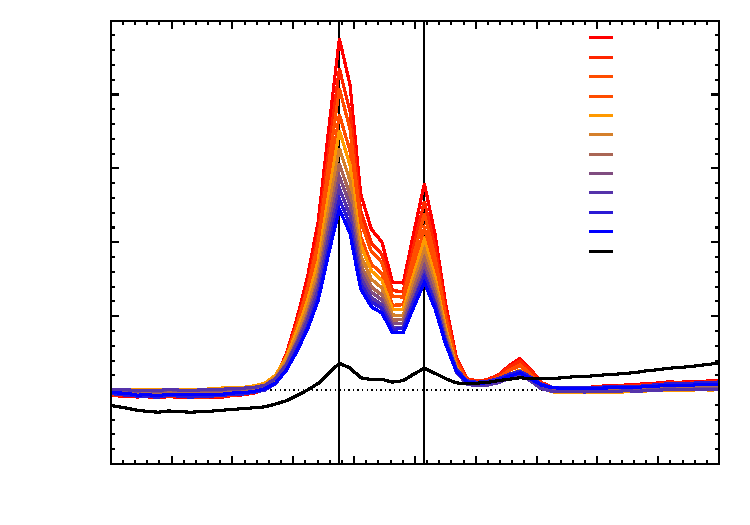
\includegraphics{pics/hdxabs}}%
    \gplfronttext
  \end{picture}%
\endgroup
